\chapter{SYSTEM DESIGN AND ANALYSIS}
\section{System Analysis}
As we know our project code-connect has to be developed in an incremental fashion or it needs to develop step by step with testing the application too. An incremental approach, also known as an iterative or step-by-step approach, is a development or problem-solving method that breaks down a larger task or project into smaller, manageable increments or steps. Rather than attempting to tackle the entire task at once, an incremental approach focuses on making incremental progress by completing and delivering smaller portions of work in a series of iterations.

Here Below are the process we need to follow
\begin{itemize}
    \setlength\itemsep{0.25em}
    \item Initial Planning and Requirements Gathering
    \item Increment Planning and Design
    \item Development and Implementation
    \item Testing and Quality Assurance
    \item Evaluation and Feedback
    \item Iterative Development and Refinement
    \item Deployment and Release
    \item Repeat the Process for Subsequent Increments
\end{itemize}
\section{Requirement Analysis}
\subsection{Functional Requirements}
The functional Requirements of our project code connect is mentioned below:
\begin{itemize}
    \item User Registration/Login:
      Users will have the option to create an account or log in using their email addresses or phone numbers. This streamlined process ensures that IT professionals can easily access the platform and connect with their peers.
    \item User Profile Management:
      Within the profile management section, users will have the ability to showcase their expertise. Portfolio management enables users to upload and highlight their project details hosted on platforms like GitHub, giving others insight into their skills and contributions. Additionally, the resume management feature allows users to present their skills, experience, and achievements in a structured manner.
    \item Connection Management:
      The platform fosters networking by allowing users to send and receive connection requests. This feature encourages the growth of professional relationships and collaboration within the IT community.
    \item Discussion/News Feed:
      The discussion and news feed serve as a dynamic space for users to share knowledge, insights, and code snippets. Users can post discussions and engage with others by 'Geeking' (similar to liking on Facebook) posts, as well as commenting to facilitate meaningful conversations.
    \item Messaging (Code Connect Messenger):
      The private messaging functionality, known as "Code Connect Messenger," enriches communication. Users can exchange private messages, fostering collaboration, mentorship, and confidential discussions within a secure environment.
    \item Notifications:
      The notifications feature keeps users engaged and informed about interactions on the platform. Users will receive notifications for activities such as receiving 'Geeks' on their posts, receiving comments, and receiving private messages. This ensures that users stay updated on relevant interactions and stay engaged with the platform's activities.
    
  \end{itemize}
\subsection{Nonfunctional Requirements}
The non functional Requirements of our project code connect is mentioned below:
\begin{itemize}
    \item Performance Enhancement: Our focus on performance involves minimizing reliance on external frameworks and modules. By reducing the use of these components, we aim to streamline the software's execution, resulting in better overall performance and responsiveness.
    \item Authentication Security: Security is a paramount concern. To enhance the platform's security, we will implement advanced authentication algorithms, particularly focusing on hashing techniques within the PHP programming environment. This ensures that user authentication data is stored and managed in a highly secure manner.
    \item Better UX Design: User experience is central to our project's success. Our emphasis on better UX design means that every aspect of the platform's interface, from navigation to interaction, will be meticulously crafted to ensure a seamless and intuitive experience. This design approach caters not only to experienced users but also to newcomers, ensuring that all users can effortlessly navigate and engage with the platform.
    \item Responsive Site: Recognizing the diverse range of devices and browsers that users utilize, we are committed to creating a responsive website. This means that the platform's design and functionality will adapt flawlessly to various screen sizes, ensuring that users can access and interact with the platform effectively, whether they are using a desktop computer, tablet, or smartphone. This responsiveness guarantees a consistent and satisfying experience across different devices and platforms, promoting accessibility and usability.
    
  \end{itemize}
\section{Feasibility Analysis}
A feasibility study is a systematic and structured analysis conducted to determine the viability and practicality of a proposed project plan. It serves as an evaluation tool to assess whether the project can be successfully implemented and if it aligns with the project's goals and objectives. It involves gathering and analyzing relevant information to determine if the project is technically feasible, operationally feasible, economically feasible, and scheduling feasible.
\subsection{Economical Feasibility}
Since the system we are developing is a web application, we will be using free and open-source software development tools such as HTML,CSS,JS, PHP, MySQL, VS Code and Figma. We will only need some economy for server for hosting if we want to host it live.
\subsection{Operational Feasibility}
Operational feasibility for the proposed system focuses ease of use. As the system is designed to be interactive, users do not require in-depth knowledge of the web app to navigate and utilize its features. The user interface (UI) is specifically designed to be user-friendly, ensuring a smooth and intuitive experience. This approach minimizes the need for extensive training and reduces potential resistance from users. Even new commers cna use it without any problem or difficulties. 
\subsection{Technical Feasibility}
There are several development technologies available. For frontend development, we have HTML,CSS,JS . For backend development, we have PHP along with the MySQL database. In our application, we have utilized HTML,CSS,JS, for the frontend and PHP with MySQL for the backend. Both HTML,CSS,JS, and PHP are open-source technologies and are supported by large companies with vibrant communities. This ensures that technical support and resources are readily available. Considering the chosen technologies and their strong community backing, the project is technically feasible.
\newpage


\subsection{Data Modelling(ER-Diagram)}
An Entity-Relationship (ER) diagram is a visual representation used to model the relationships between various entities in a database. It's a graphical way of showing the structure of a database, focusing on the entities (objects) within the system and how they relate to each other. ER diagrams are widely used in database design and conceptual modeling to help designers and stakeholders understand the data and its relationships.
\begin{figure}[H]
    \rotatebox{90}{
    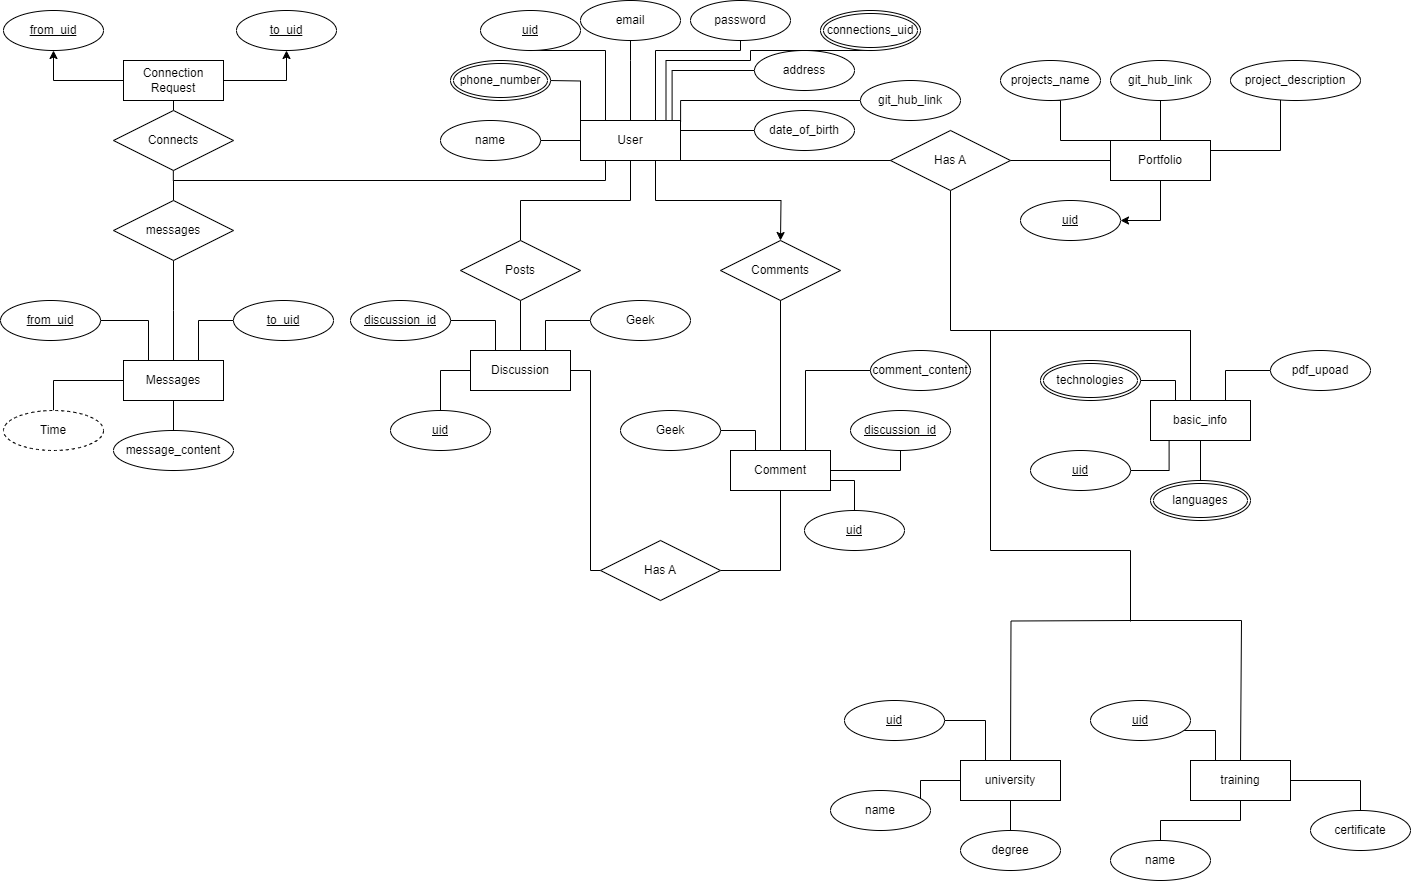
\includegraphics[height = 15cm]{Diagrams/er.drawio.png}}
    \caption{ER Diagram of System Data}
\end{figure}
\newpage
\subsection{DFD}
DFD or Data Flow Diagram is mainly used to show how data are being flowed in and out of our system. There are 3 levels of DFD i.e Context Level(Level 0),Level 1 and Level 2
\begin{figure}[H]
    \centering
    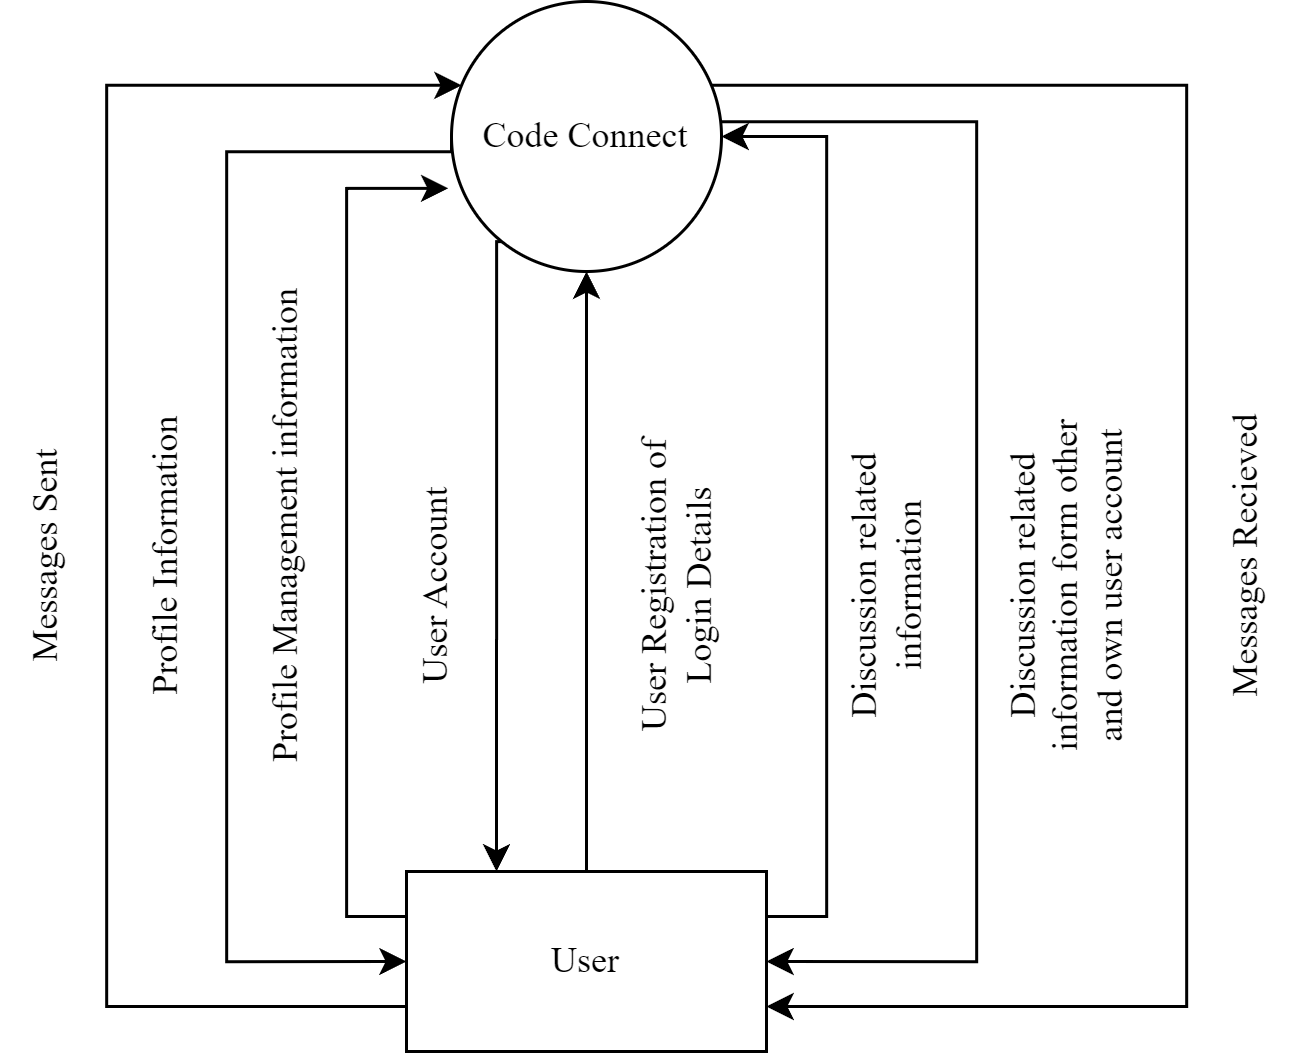
\includegraphics[height = 8cm]{Diagrams/DFD.drawio.png}
    \caption{Data Flow Diagram (Context Level)}
\end{figure}
\newpage
\section{System Design}
\subsection{Architecture Design}
The following diagram shows diagram of our Architecture. Mainly shows what are the functions can be accessed after starting our application.
\begin{figure}[H]
    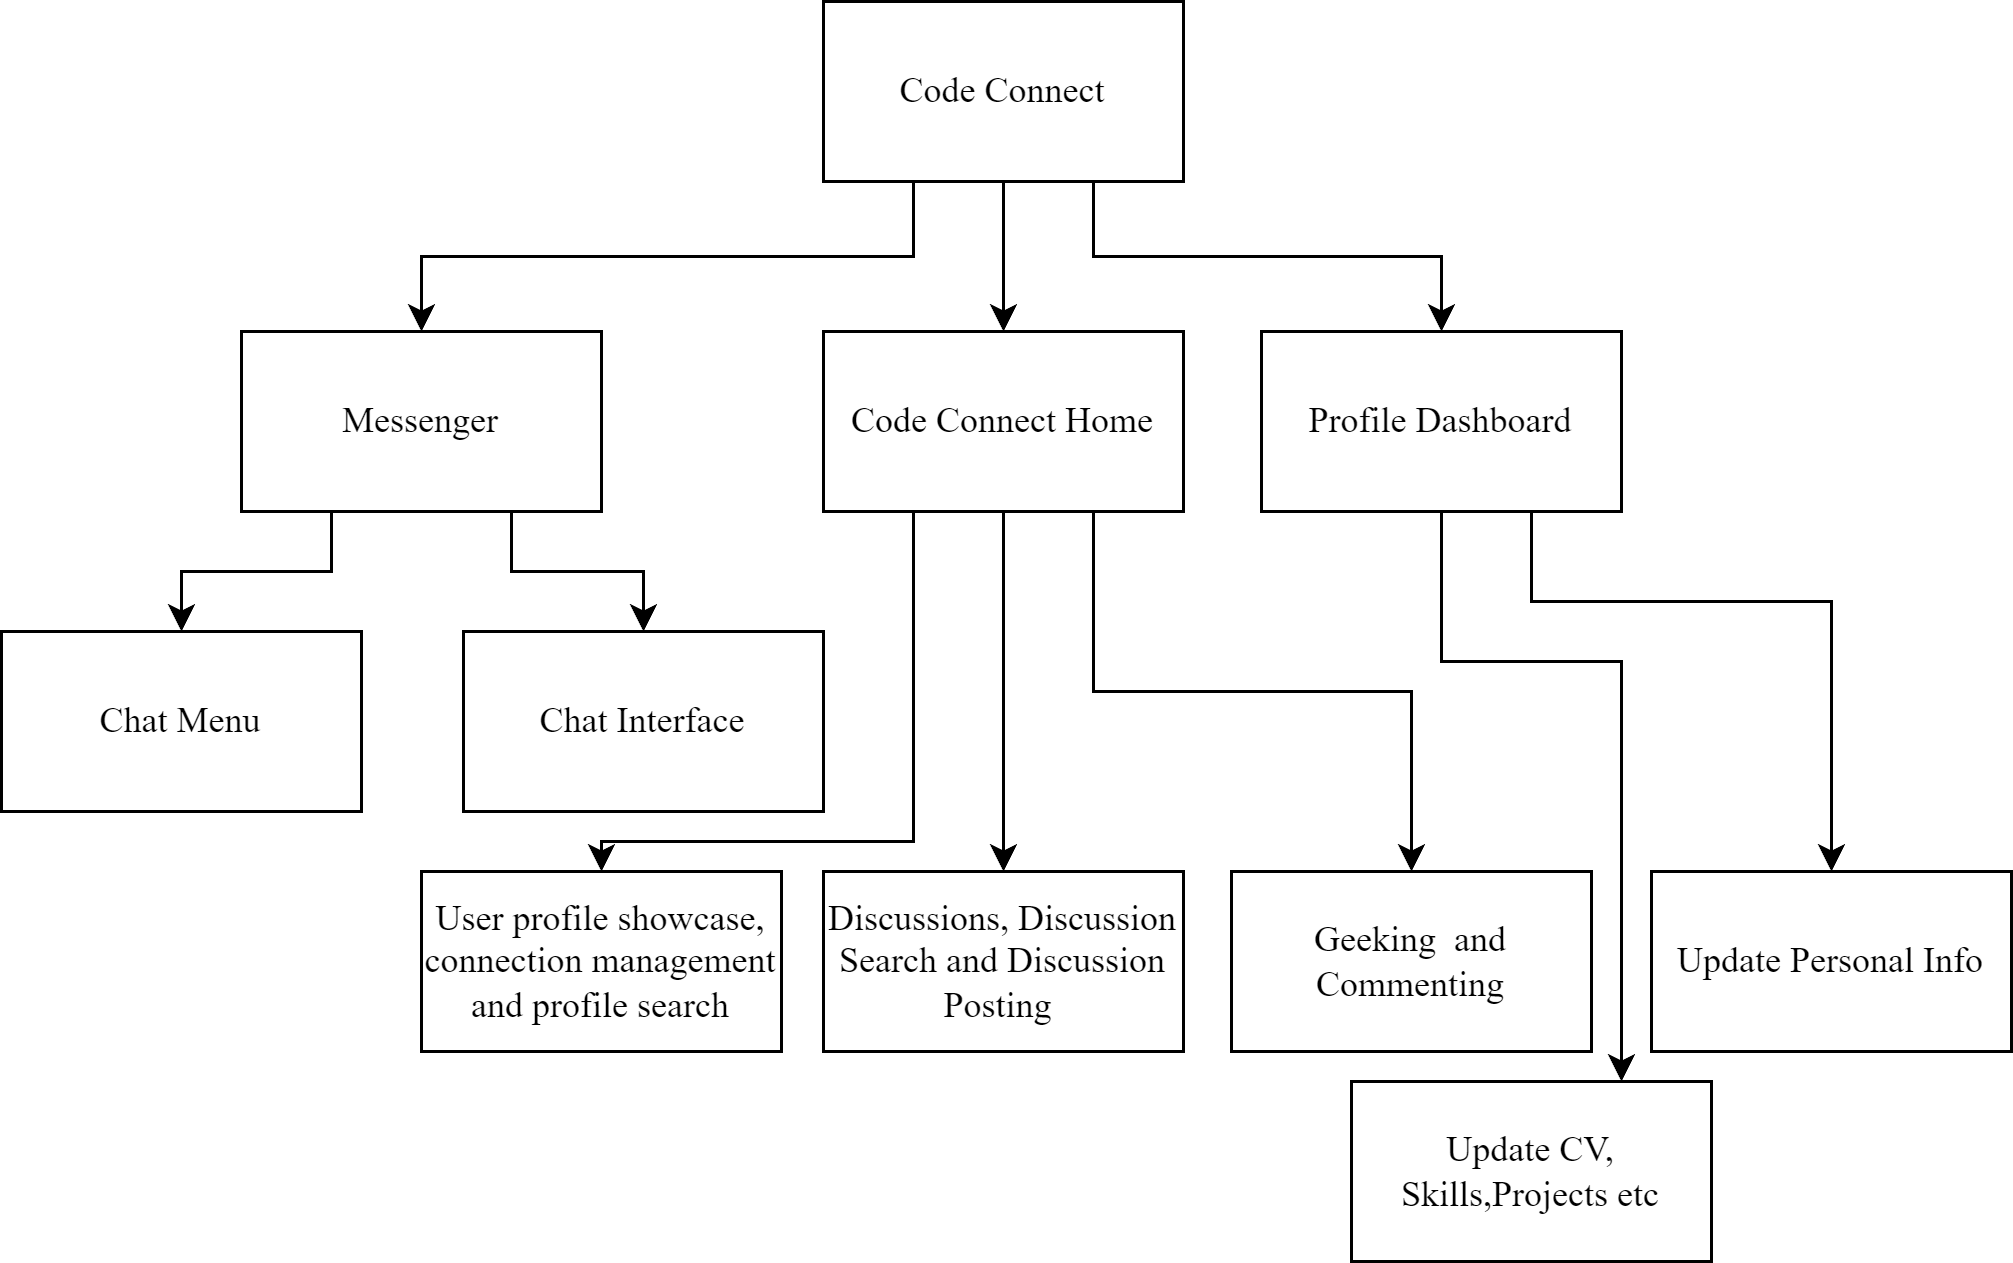
\includegraphics[height = 8cm]{Diagrams/Main_Block.png}
    \caption{Main Architecture of System}
\end{figure}
% \newpage
% \subsection{Activity Diagram}
% An activity diagram visually presents a series of actions or flow of control in a system similar to a flowchart or a data flow diagram. This diagram showed how our program flow goes on.
% \begin{figure}[H]
%    \centering
%     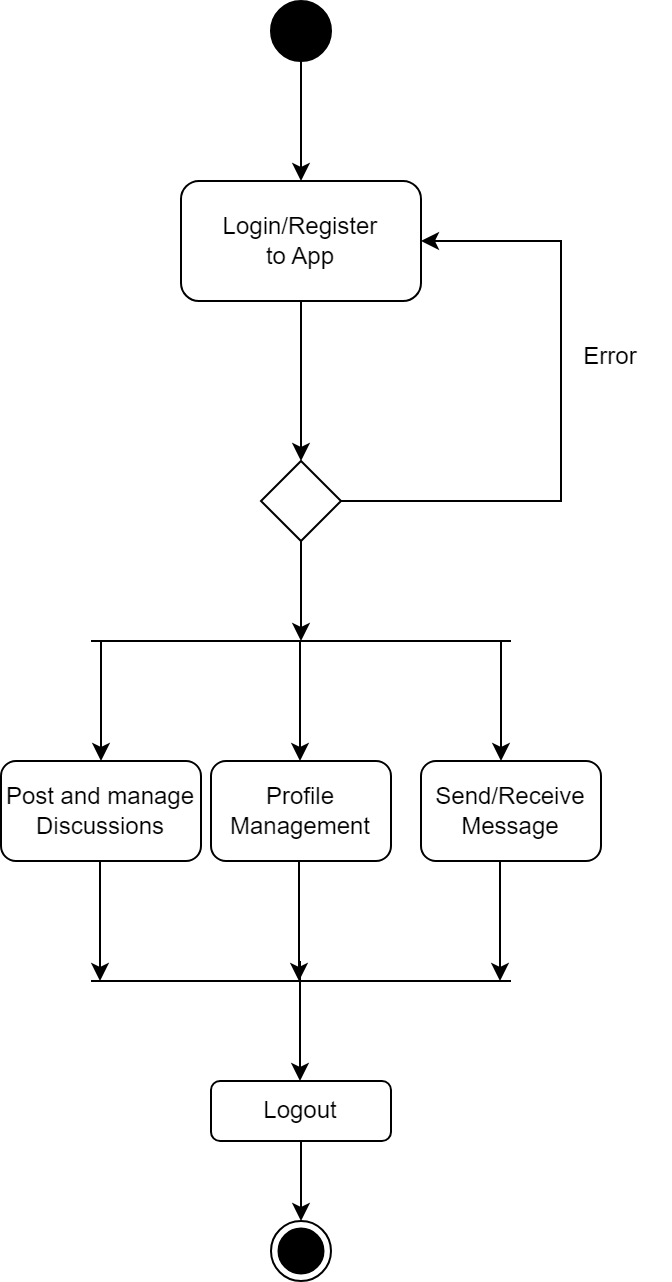
\includegraphics[height = 15cm]{Diagrams/Activity.drawio.png}
%     \caption{Activity Diagram}
% \end{figure}
\newpage
\subsection{Schema Design}
Schema design, in the context of software development and database management, refers to the process of creating a structure or blueprint that defines how data will be organized, stored, and related within a database. It involves making decisions about how different types of data will be represented, how they will be interconnected, and how the database will efficiently retrieve and store information.
\begin{figure}[H]
    \centering
    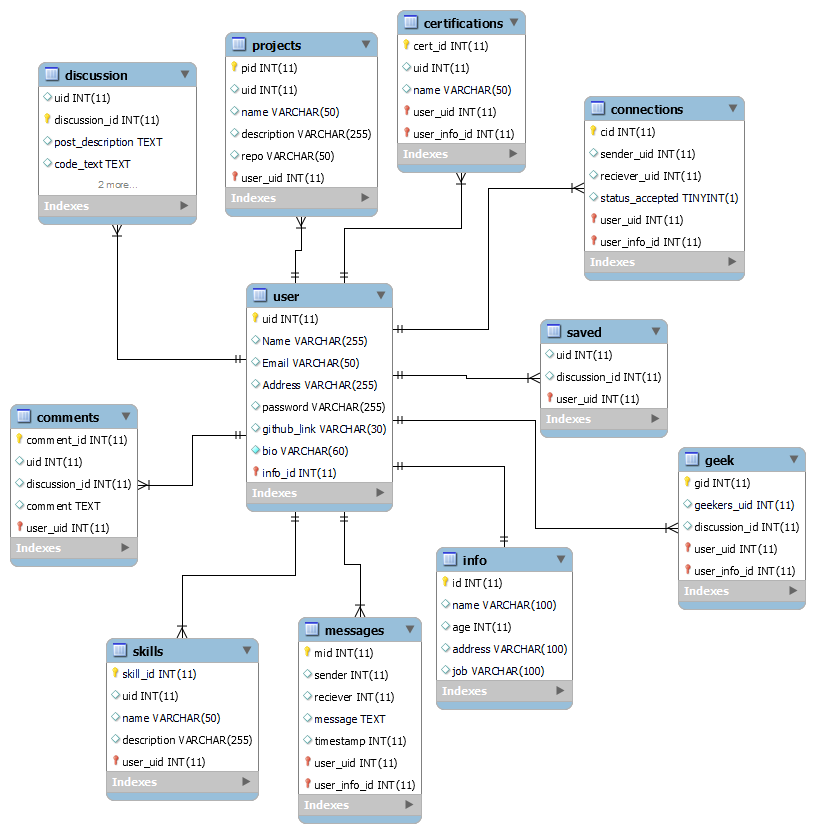
\includegraphics[height = 13cm]{Diagrams/schema.png}
    \caption{Database Schema Design}
\end{figure}
\newpage
\subsection{Interface Design}
\subsubsection{Usere Interface Design}
User interface (UI) design refers to the process of creating the visual layout and elements that users interact with when using a software application, website, or any digital product. UI design focuses on making the user experience intuitive, visually appealing, and user-friendly. 
\begin{figure}[H]
    \centering
    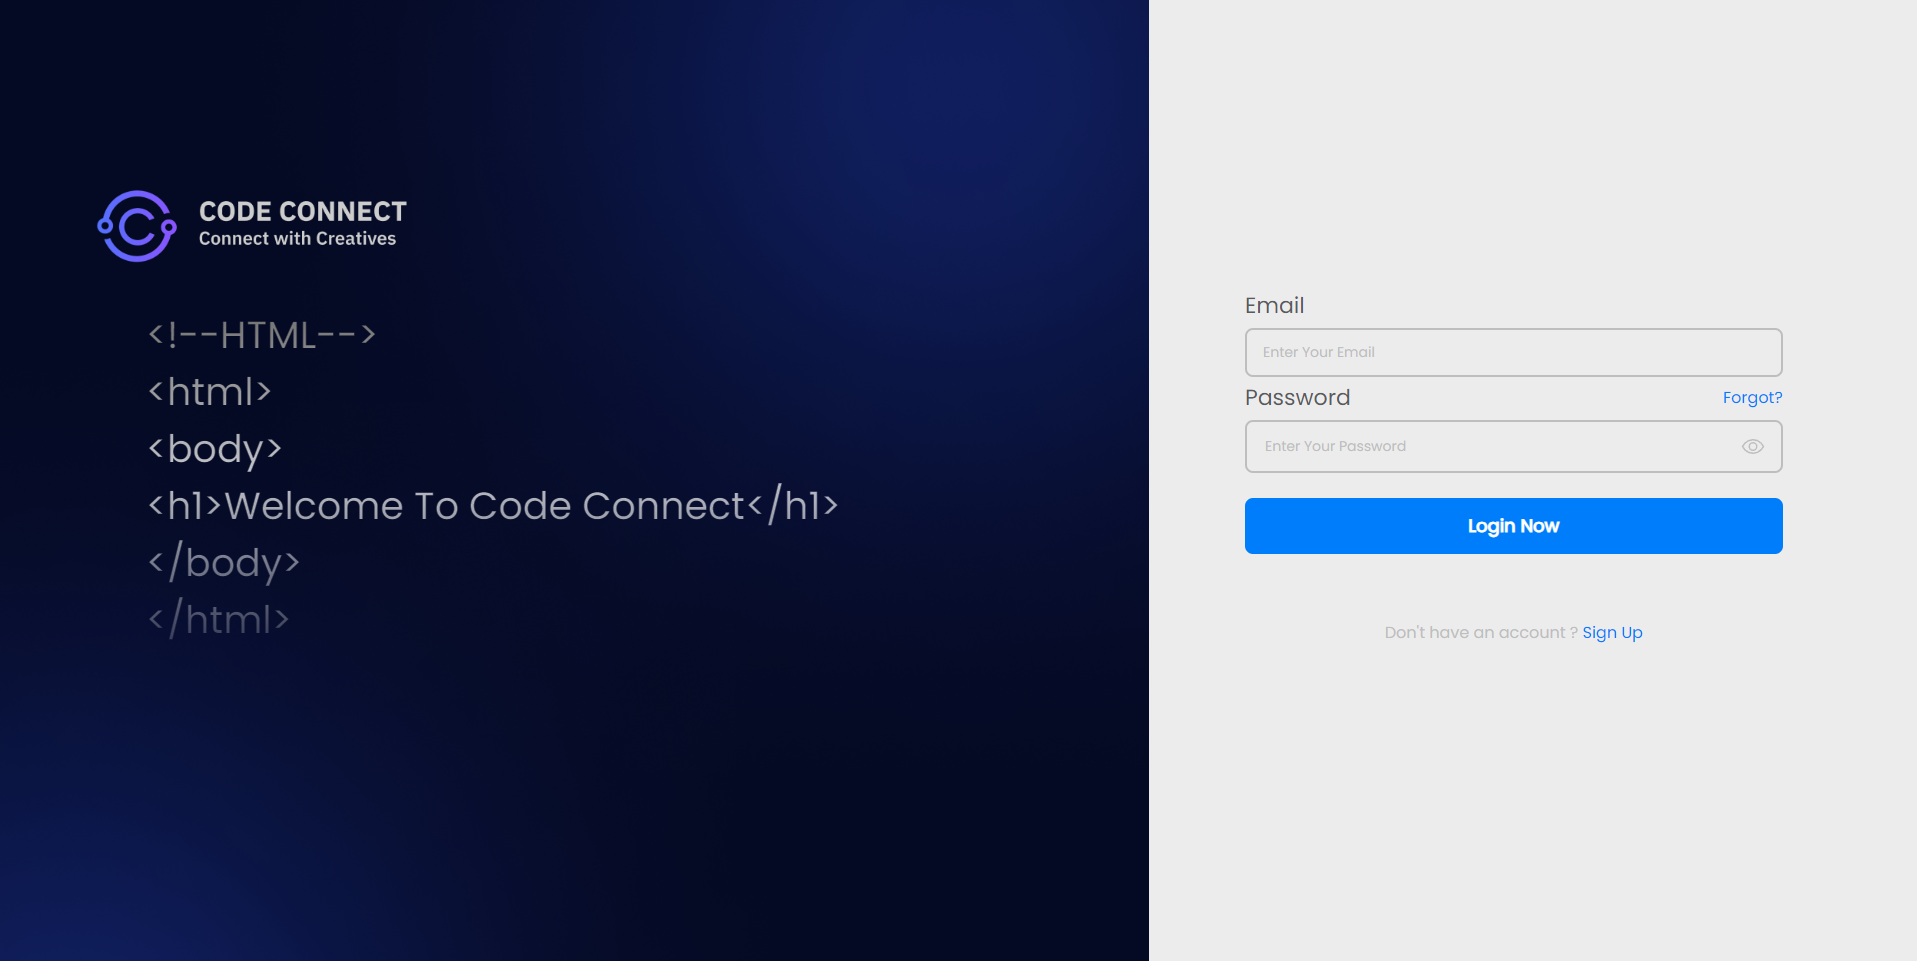
\includegraphics[height = 7cm]{ui_diagrams/desktop_login.png}
    \caption{Desktop Login UI}
\end{figure}
\begin{figure}[H]
  \centering
  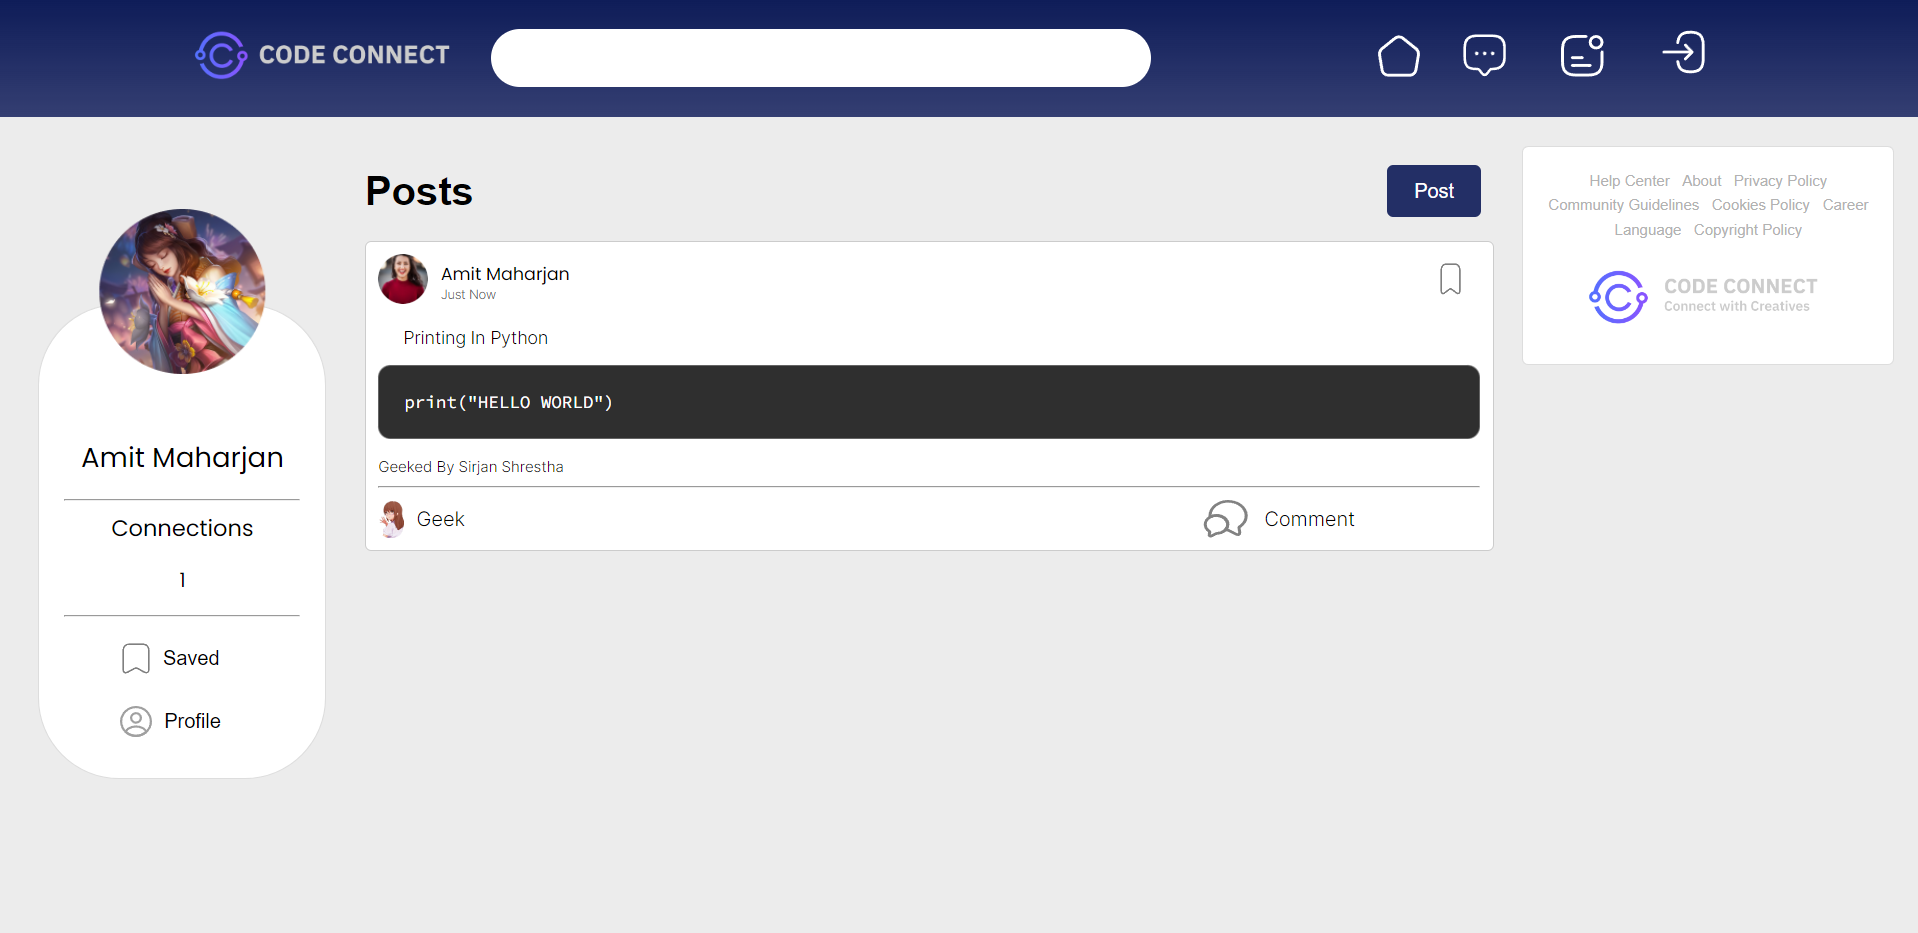
\includegraphics[height = 6.8cm]{ui_diagrams/desktop_homepage.png}
  \caption{Desktop Homepage UI}
\end{figure}
\begin{figure}[H]
  \centering
  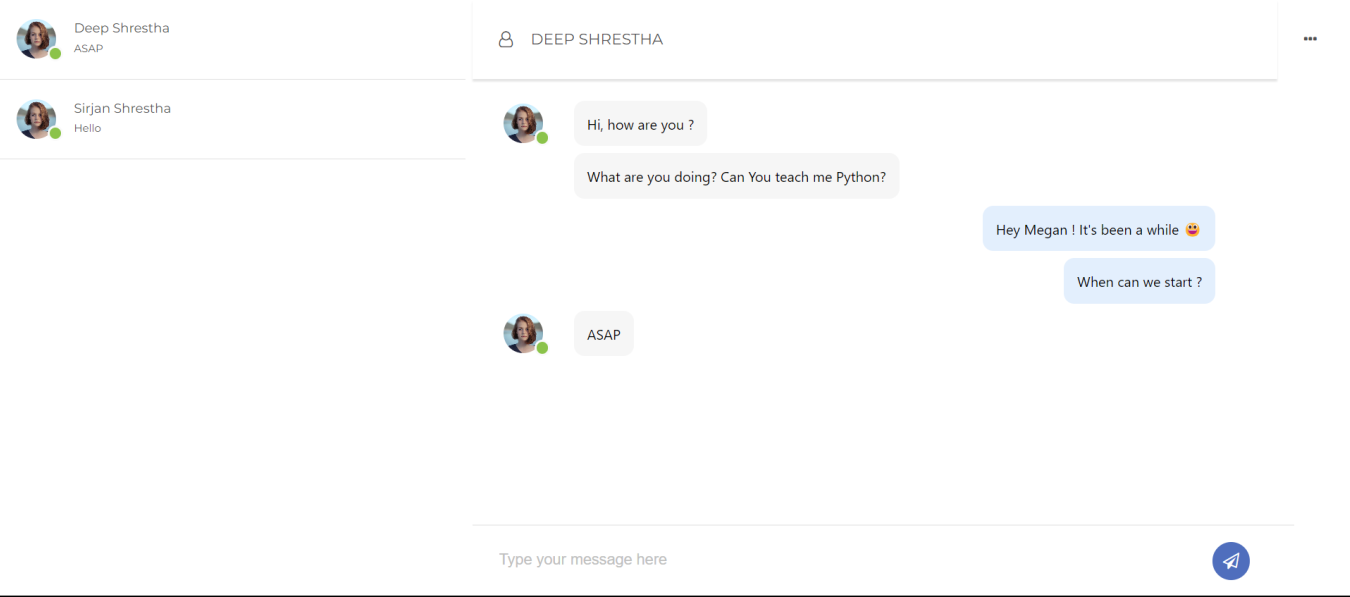
\includegraphics[height = 6.8cm]{ui_diagrams/desktop_messages.png}
  \caption{Desktop Messages UI}
\end{figure}
\begin{figure}[H]
  \centering
  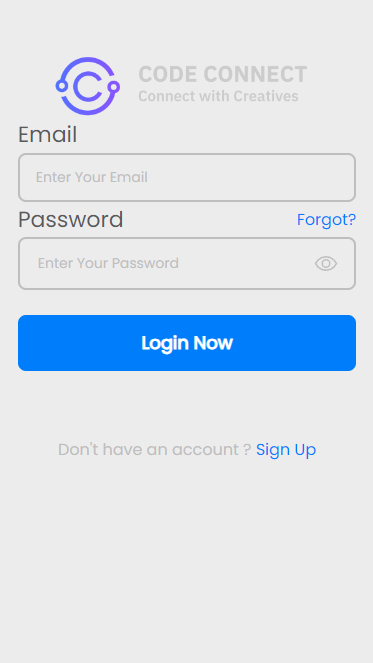
\includegraphics[height = 8cm]{ui_diagrams/mobile_login.png}
  \caption{Mobile Login UI}
\end{figure}
\newpage
\subsection{Physical DFD}
A Physical Data Flow Diagram (DFD) is a graphical representation of how data flows within a system at a more detailed and implementation-oriented level than a logical DFD. While a logical DFD focuses on the system's functional aspects and processes, a physical DFD includes details about how data is processed, where it's stored, and how it's transferred between system components.
\begin{figure}[H]
  \rotatebox{90}{
  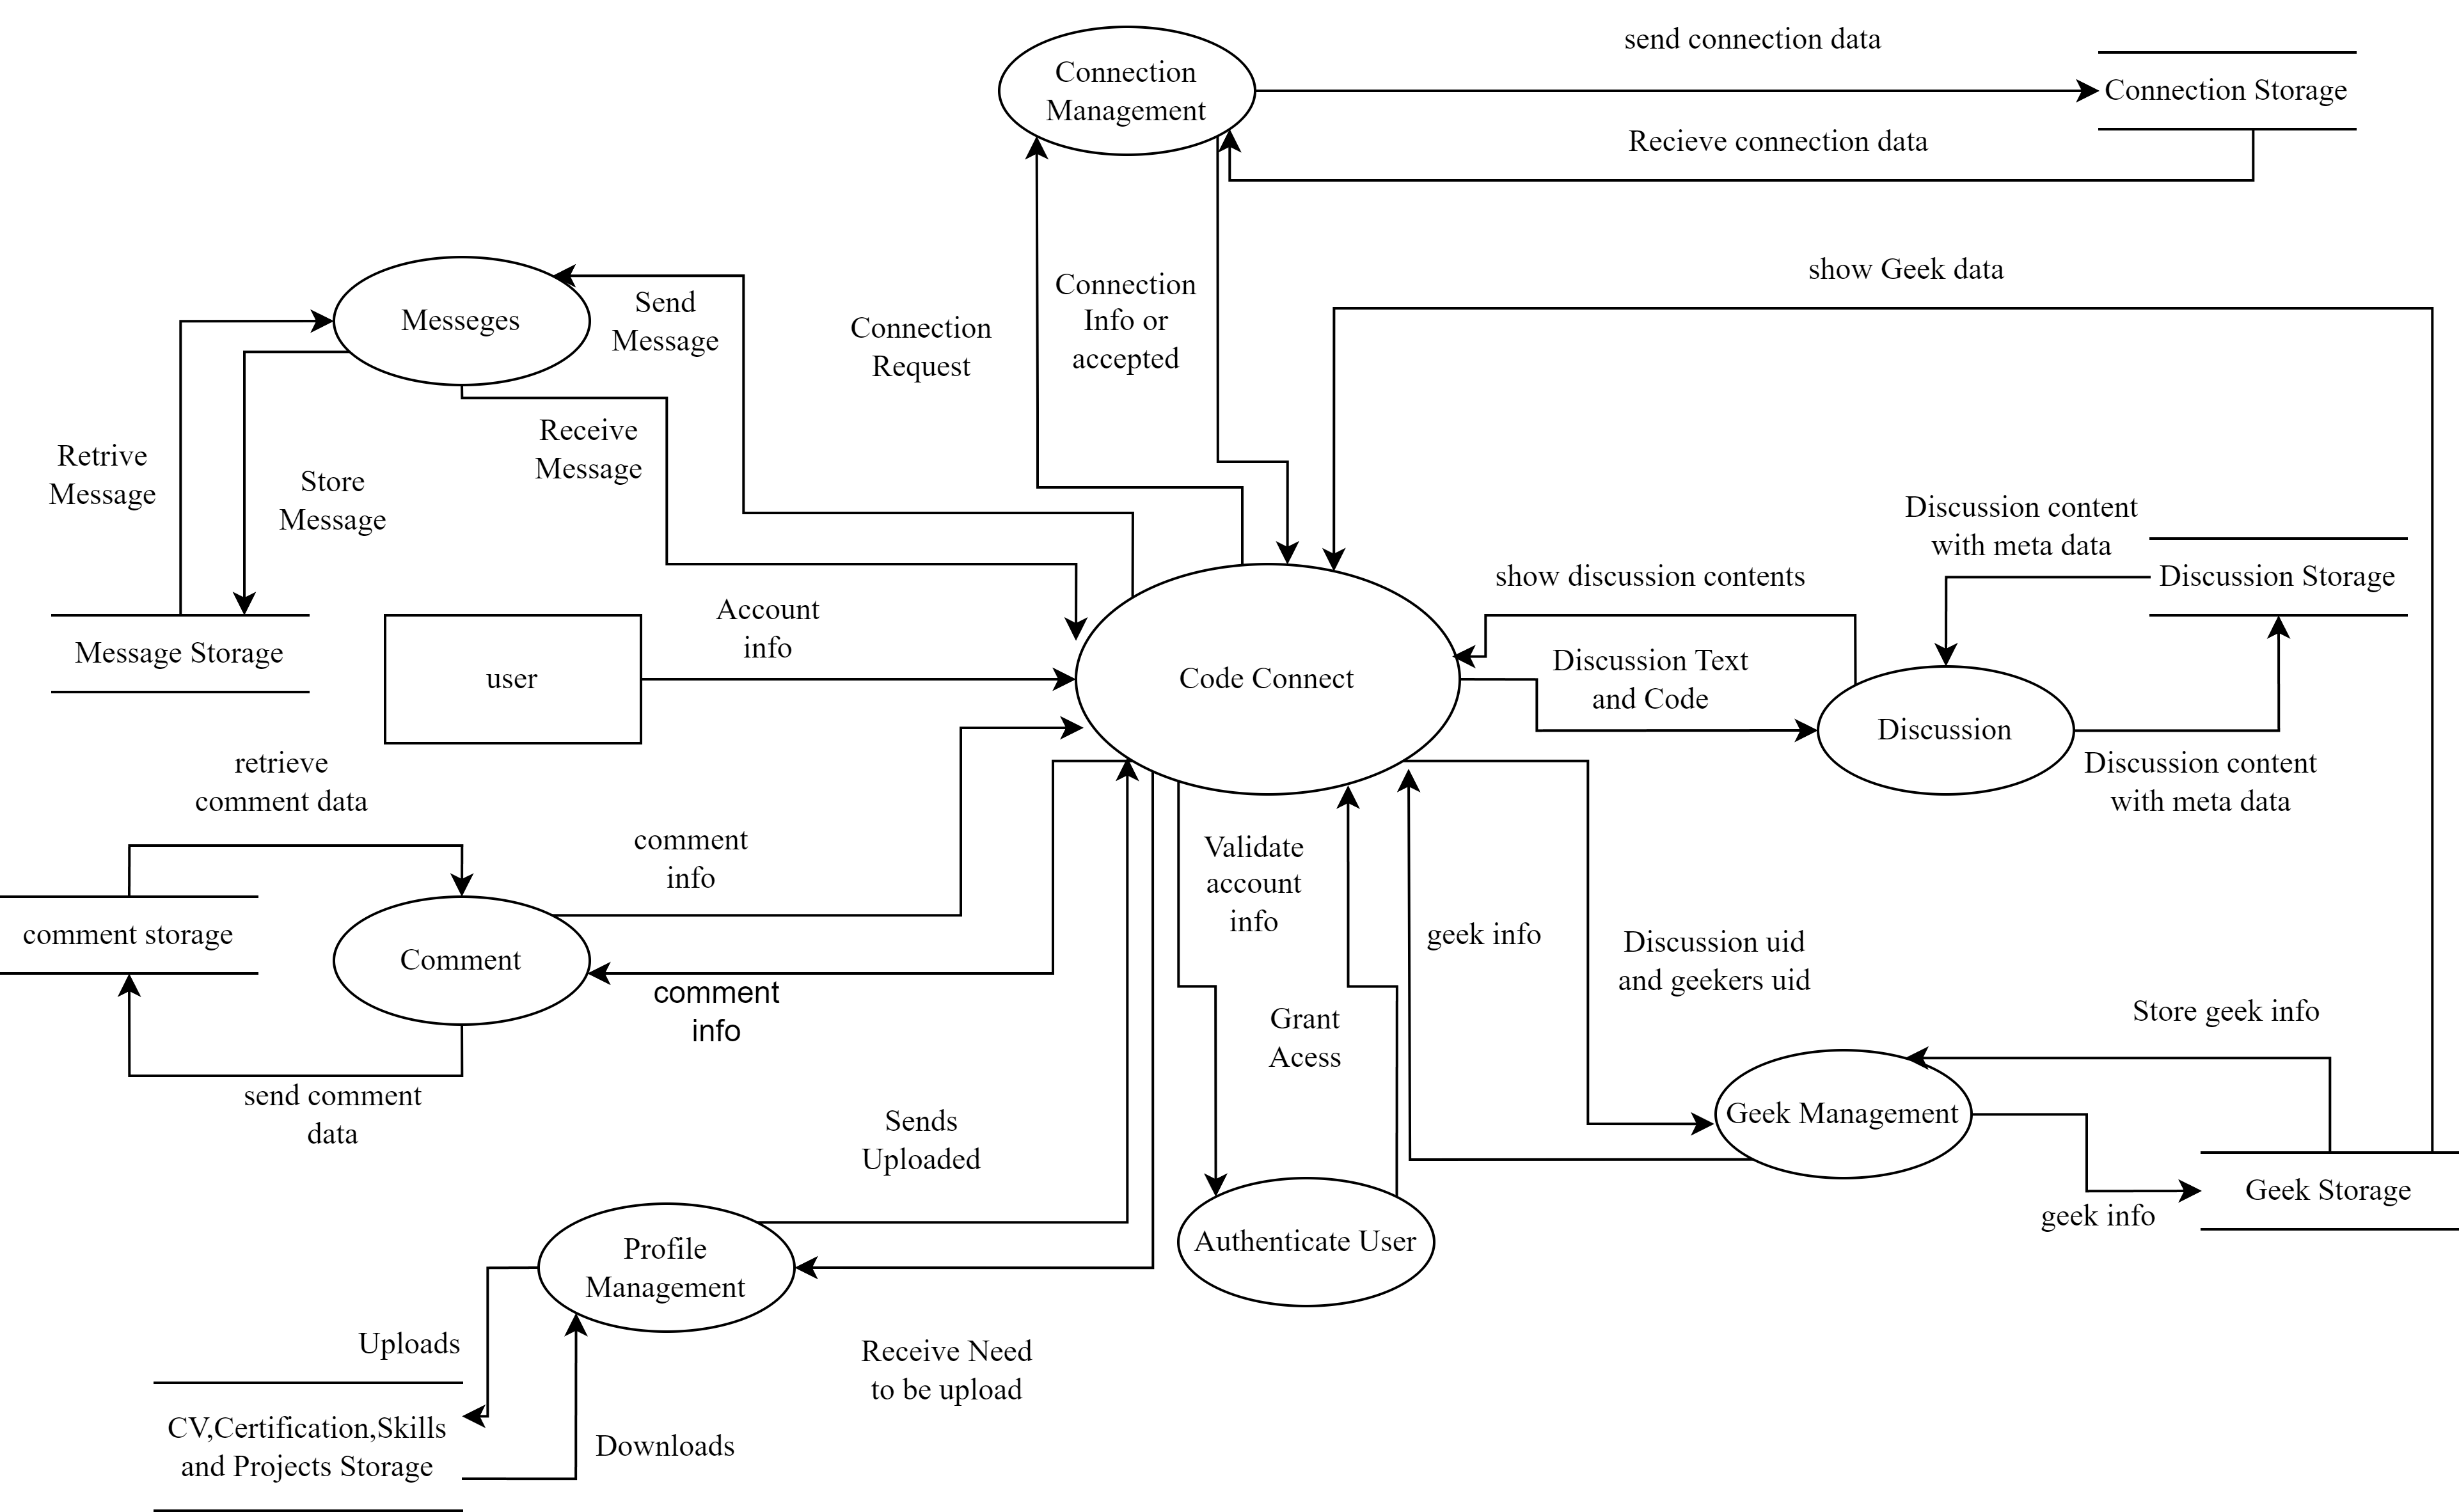
\includegraphics[height = 8cm]{Diagrams/physical_dfd.png}}
  \caption{ER Diagram of System Data}
\end{figure}
\newpage